\documentclass[dissertation.tex]{subfiles}
\begin{document}

\chapter{Exploration of learned representations}

\section{Token-level embeddings}

Filter to notes

\begin{figure}[htpb]
    \centering
    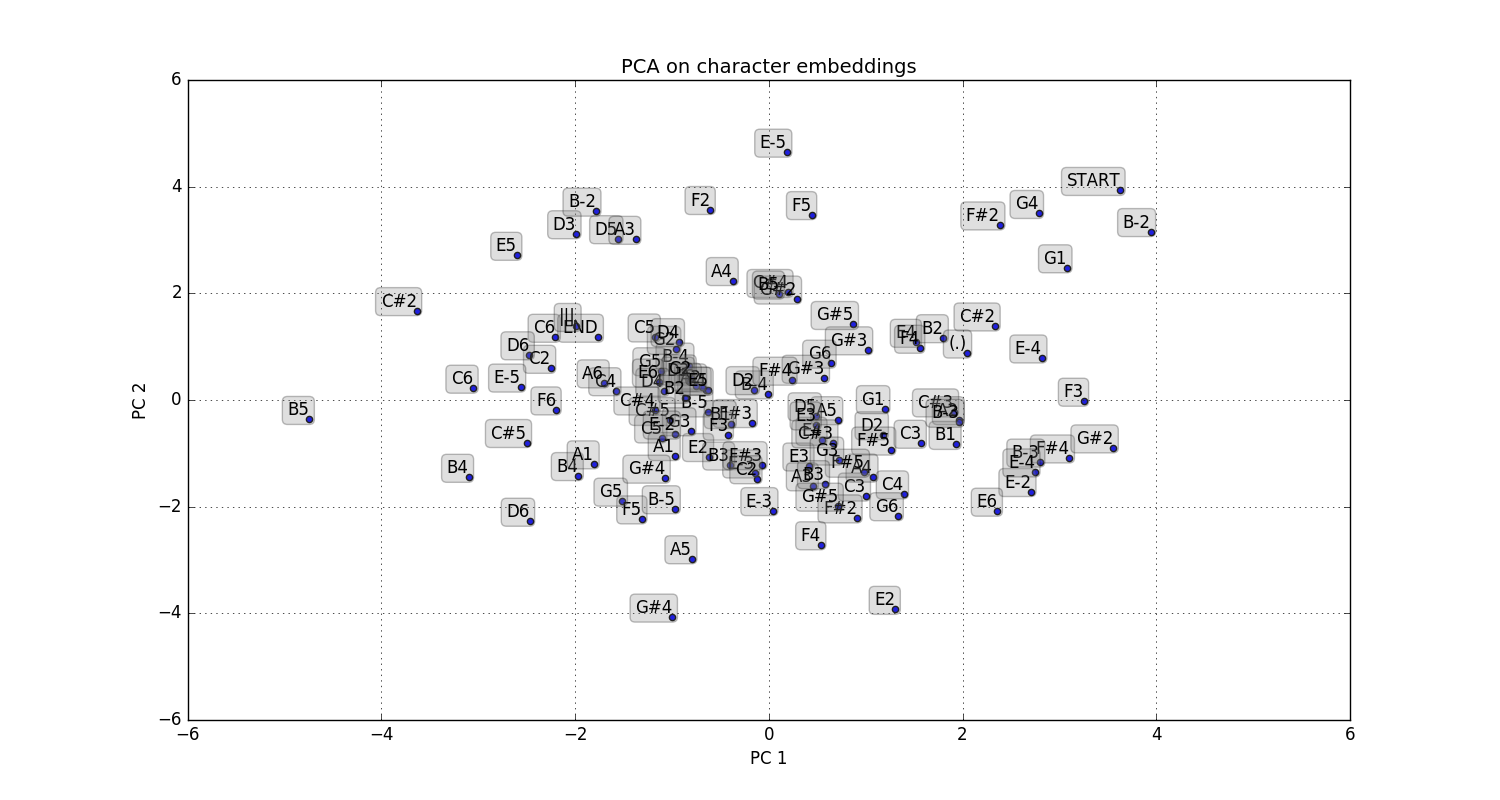
\includegraphics[width=1.0\linewidth]{Figures/PCA-notes.png}
    \caption{PCA embedding of note tokens}
    \label{fig:pca-notes}
\end{figure}

\begin{figure}[htpb]
    \centering
    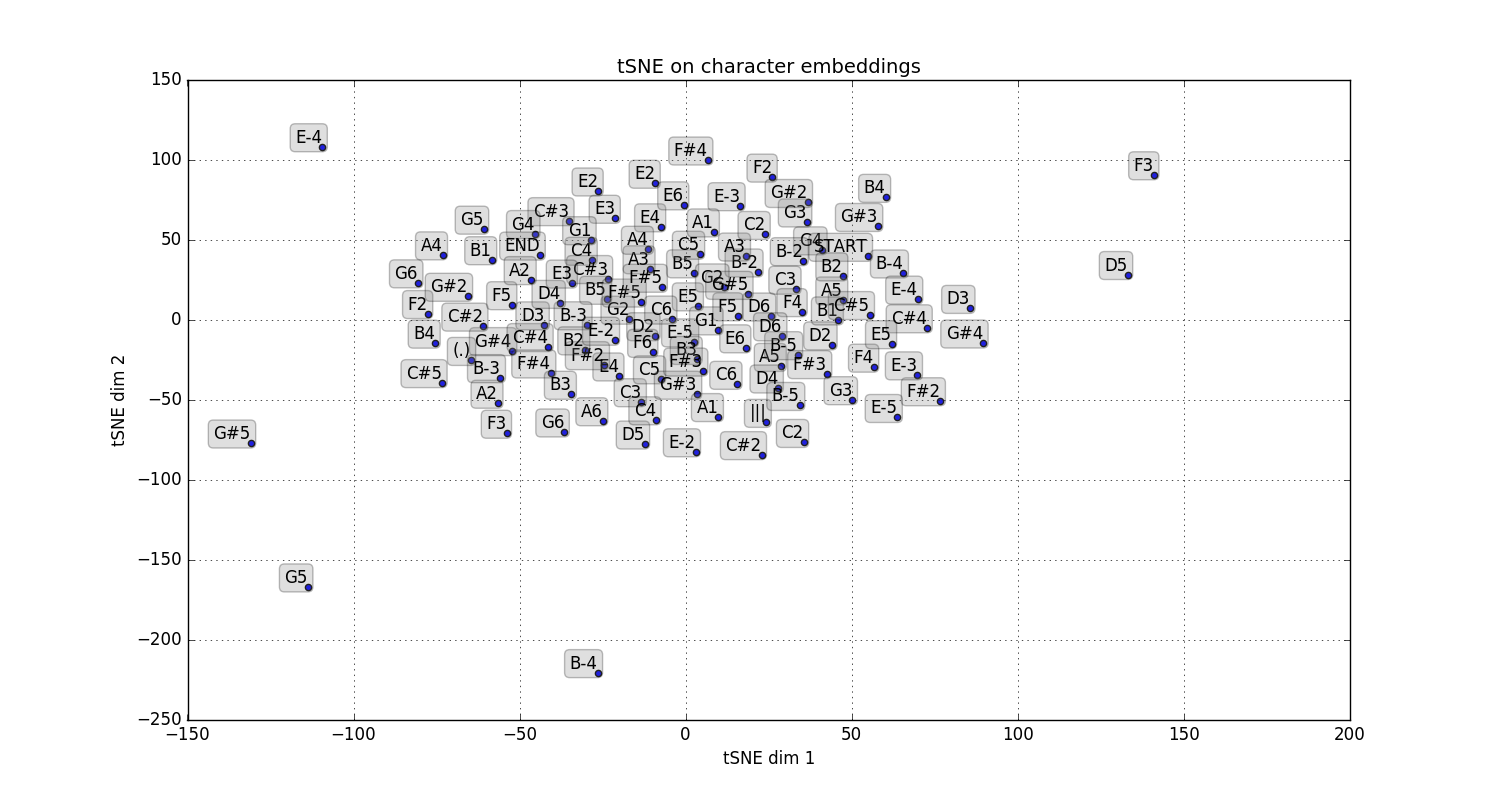
\includegraphics[width=1.0\linewidth]{Figures/tSNE-notes.png}
    \caption{tSNE embedding of note tokens}
    \label{fig:tsne-notes}
\end{figure}

\subsection{Variable-length embeddings}

\todo{LSTM hidden state after consuming chord (chord boundary, do they
    cluster?), phrase (up to fermata, do similar phrases embed similarly),
    whole pieces (difficult to evaluate)}

\section{LSTM Layer activations}

Inputs

\begin{figure}[htpb]
    \centering
    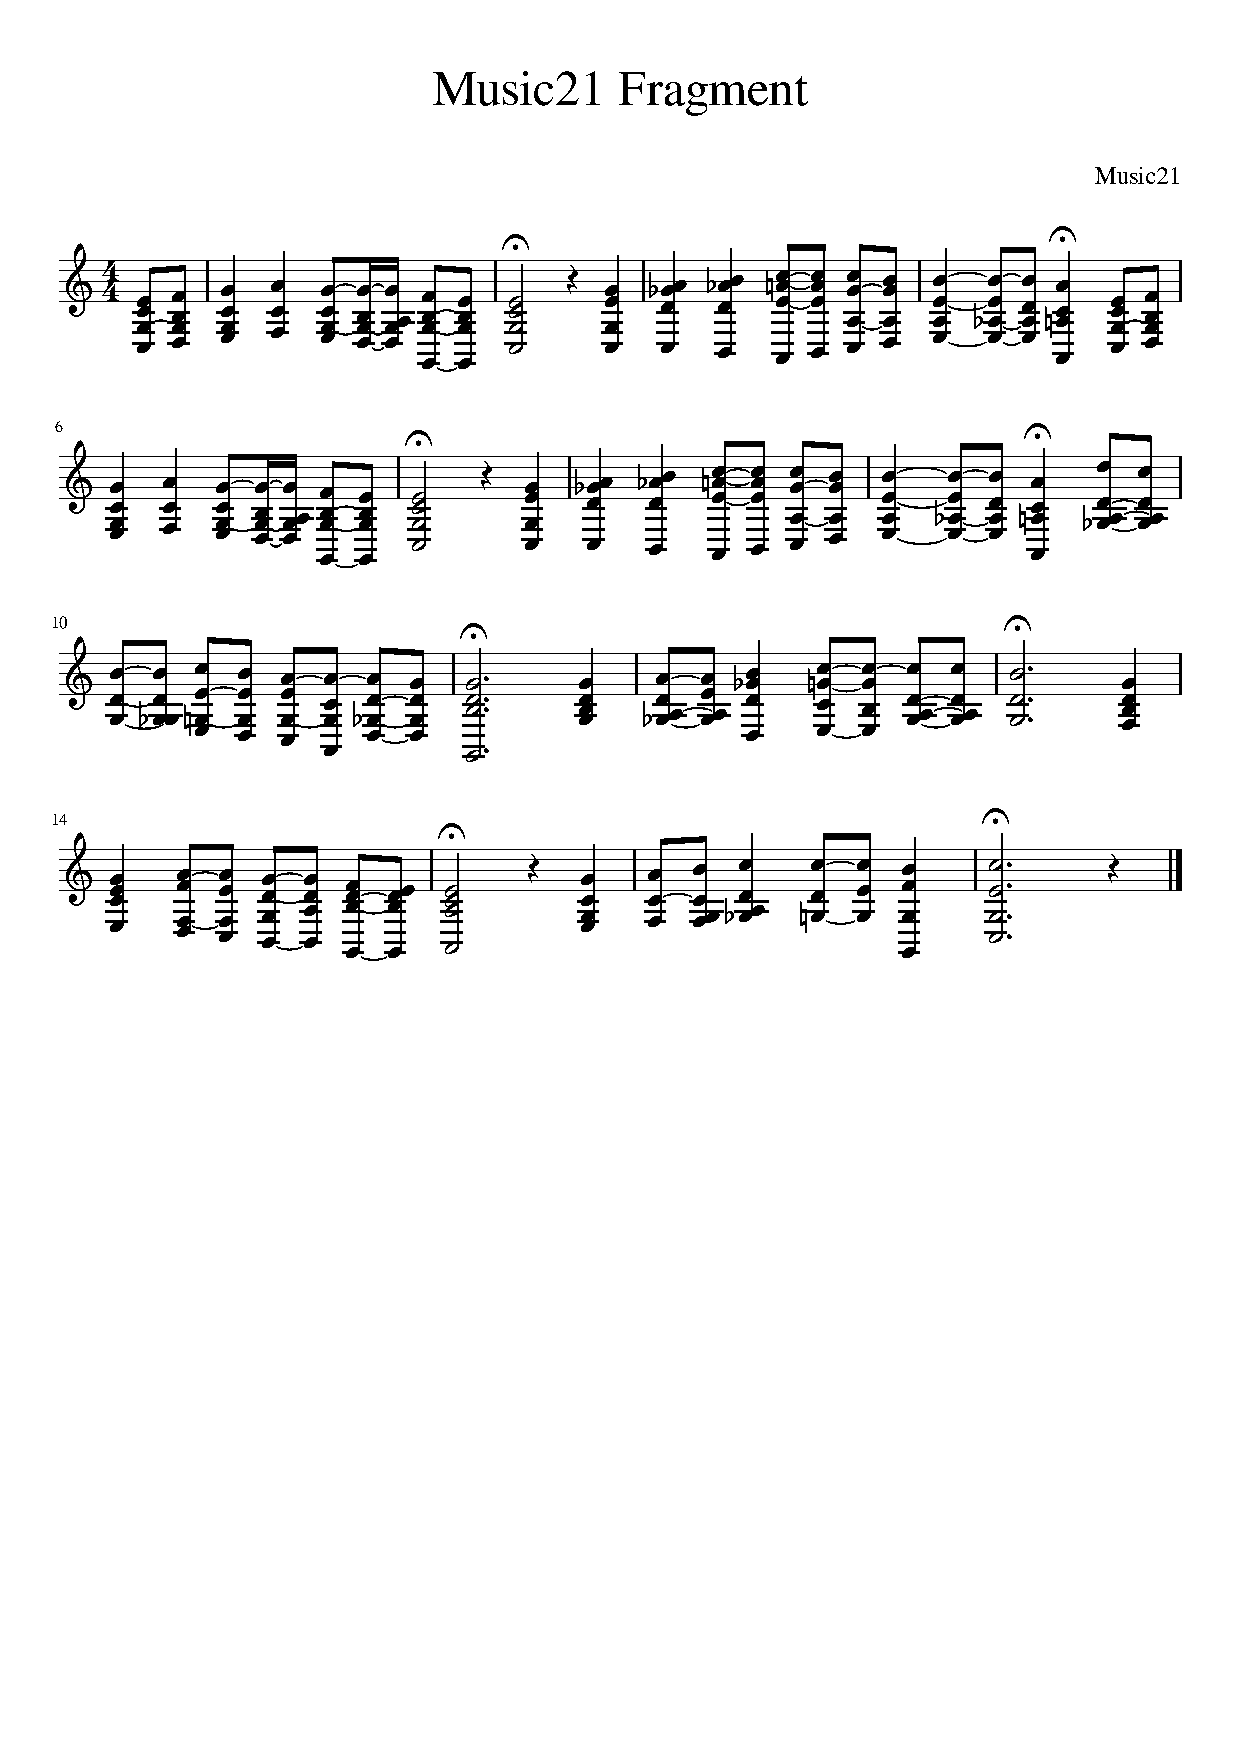
\includegraphics[trim={0 13cm 0 3.5cm},clip,width=0.95\linewidth]{Figures/model-analysis-input-score.pdf}
    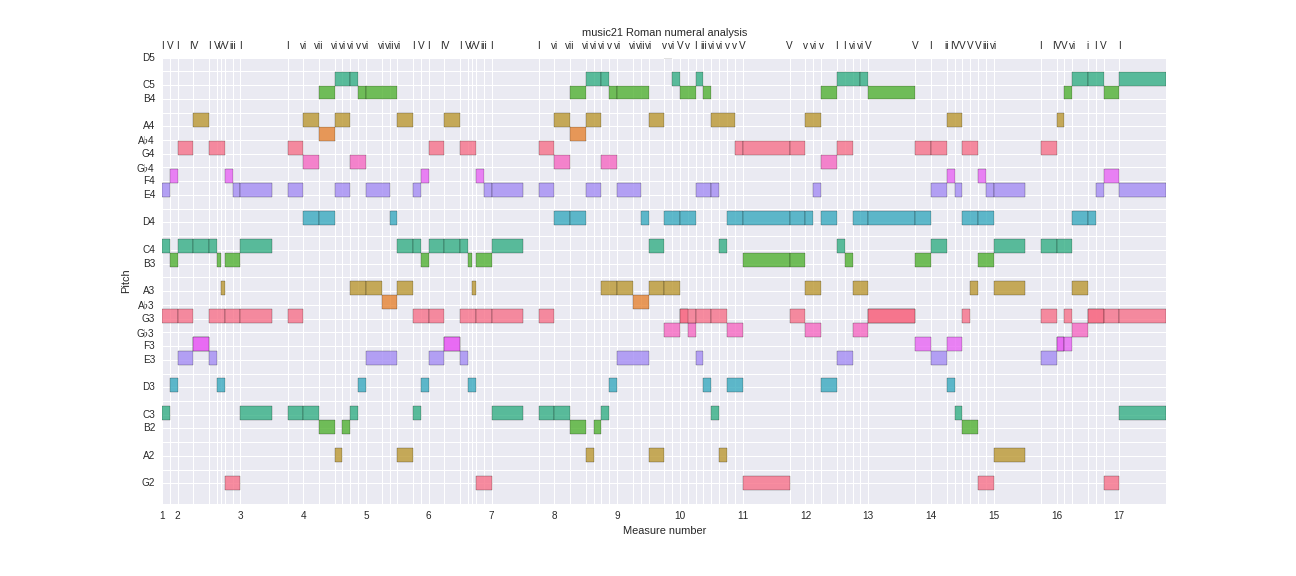
\includegraphics[width=1.0\linewidth]{Figures/model-analysis-input-piano-roll.png}
    \caption{}
    \label{fig:}
\end{figure}

Network activations

\begin{figure}[htpb]
    \centering
    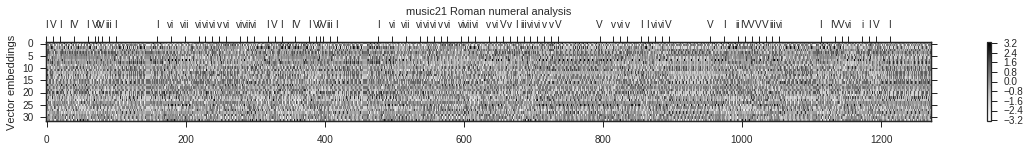
\includegraphics[width=1.0\linewidth]{Figures/model-analysis-tokens-0.png}
    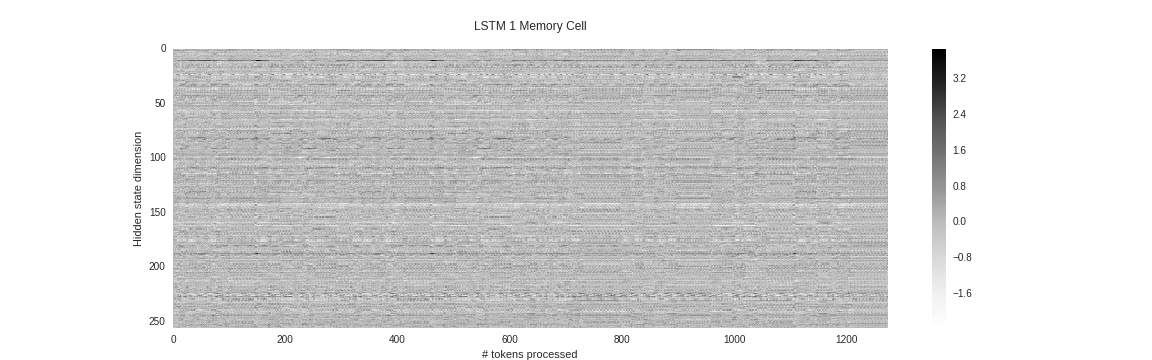
\includegraphics[width=1.0\linewidth]{Figures/model-analysis-tokens-1.png}
    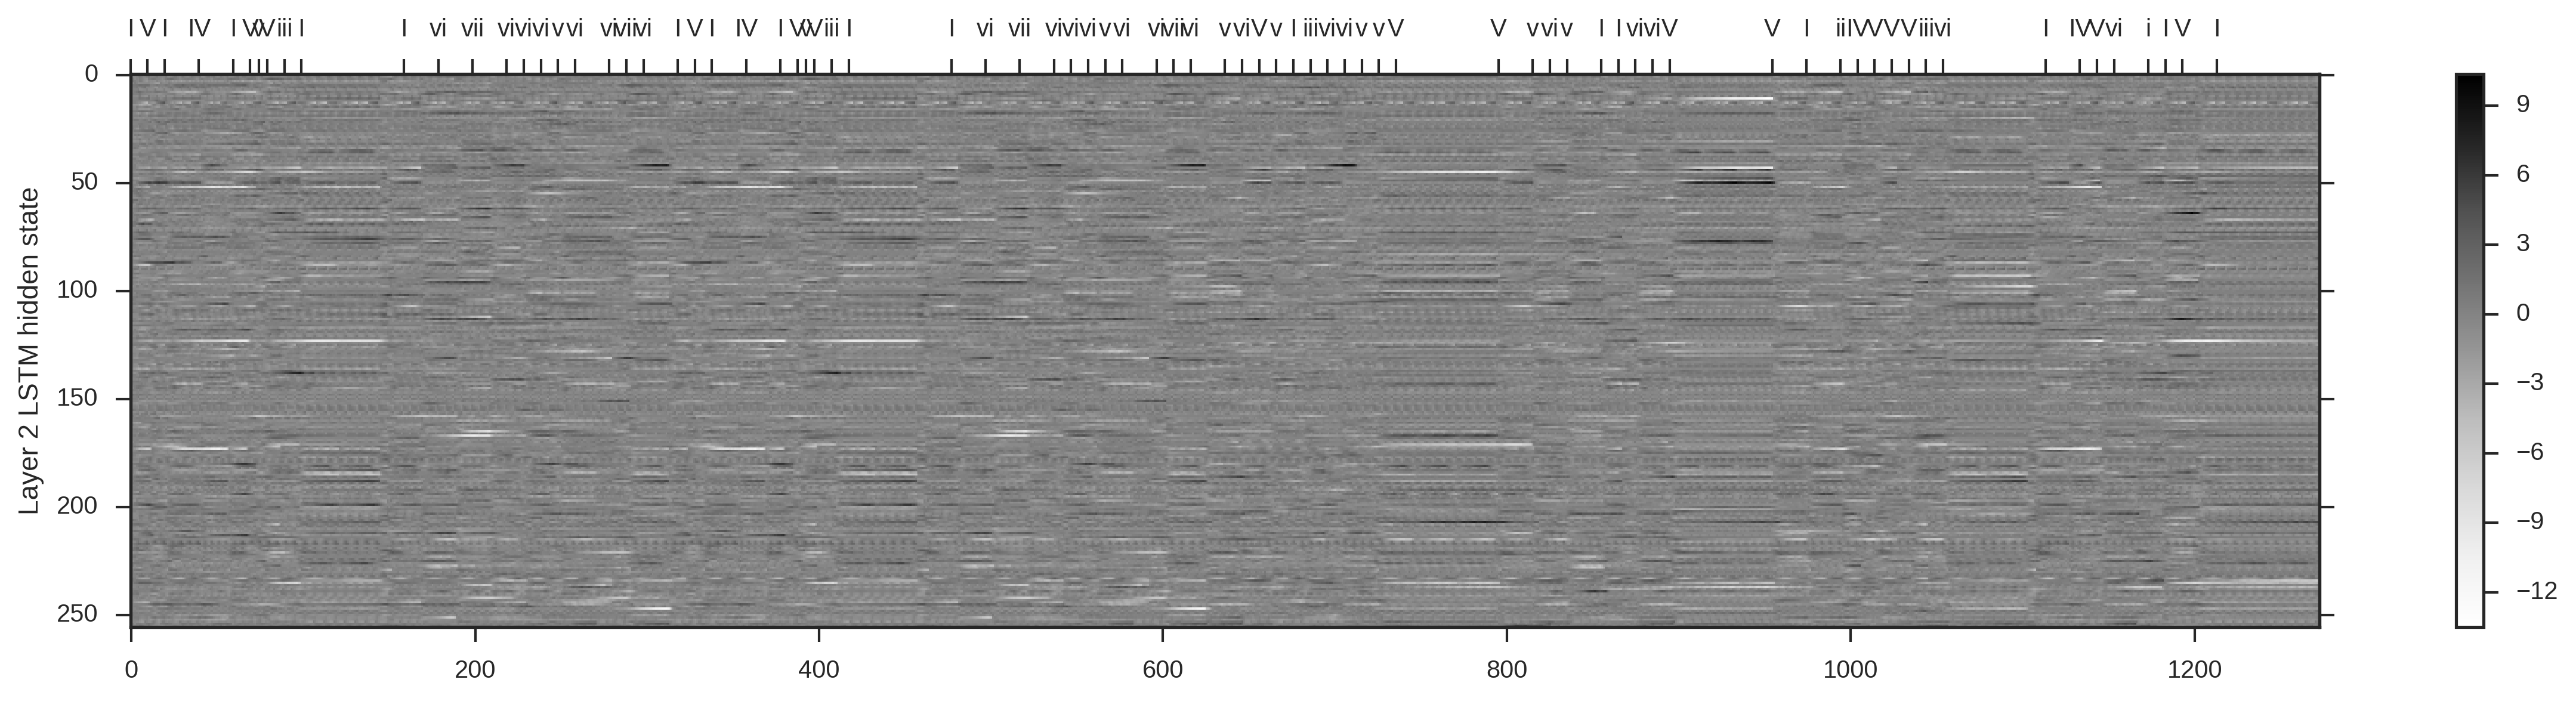
\includegraphics[width=1.0\linewidth]{Figures/model-analysis-tokens-2.png}
    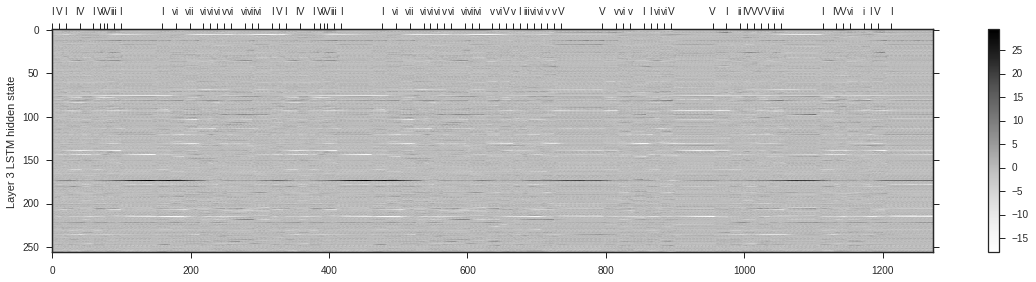
\includegraphics[width=1.0\linewidth]{Figures/model-analysis-tokens-3.png}
    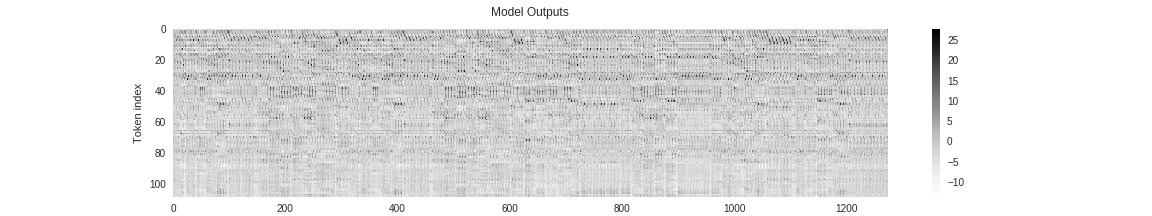
\includegraphics[width=1.0\linewidth]{Figures/model-analysis-tokens-4.png}
    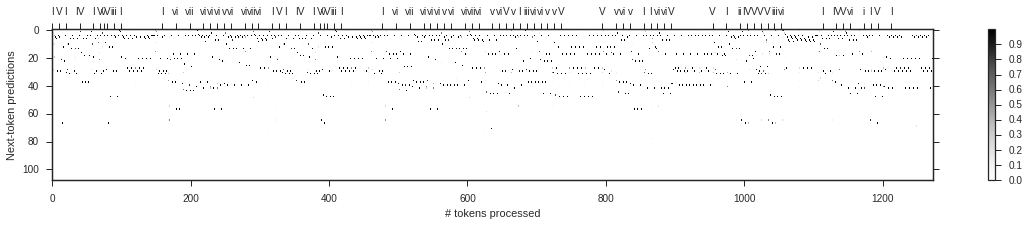
\includegraphics[width=1.0\linewidth]{Figures/model-analysis-tokens-5.png}
    \caption{}
    \label{fig:}
\end{figure}

Pooling over chords
\begin{figure}[htpb]
    \centering
    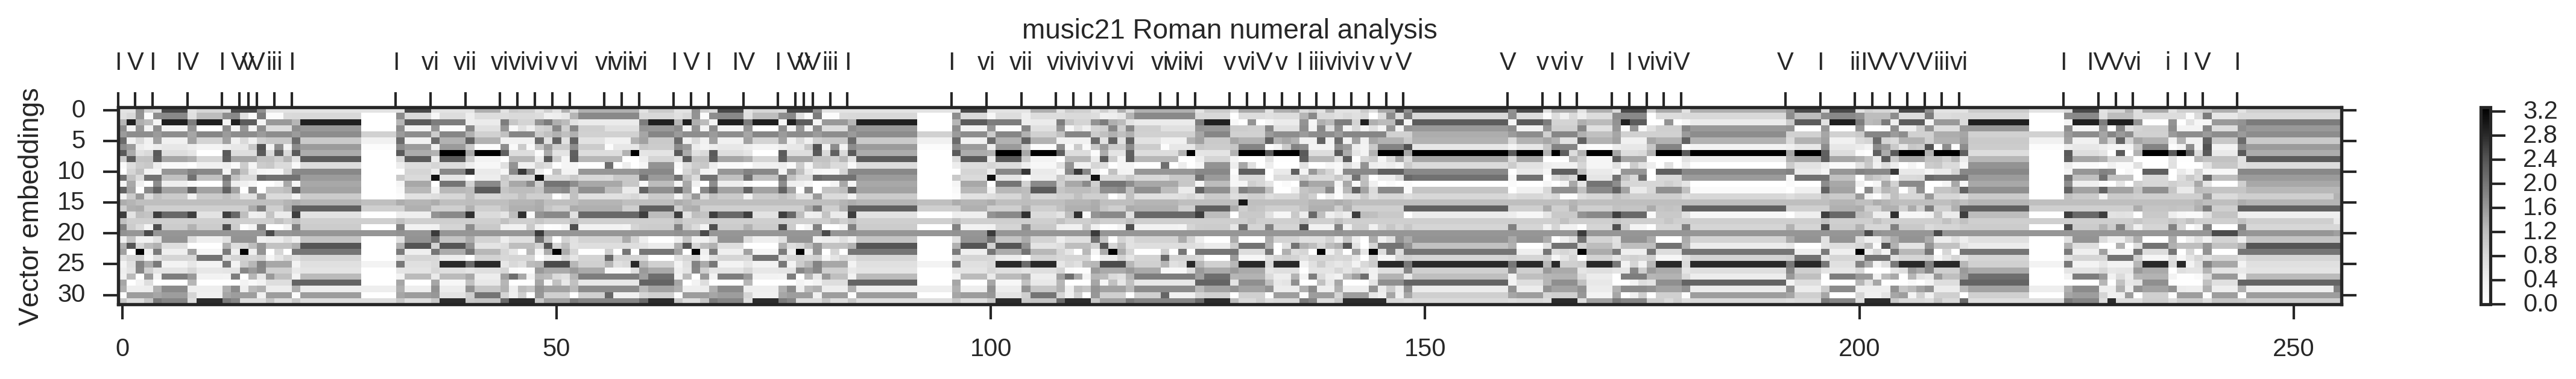
\includegraphics[width=1.0\linewidth]{Figures/model-analysis-chords-0.png}
    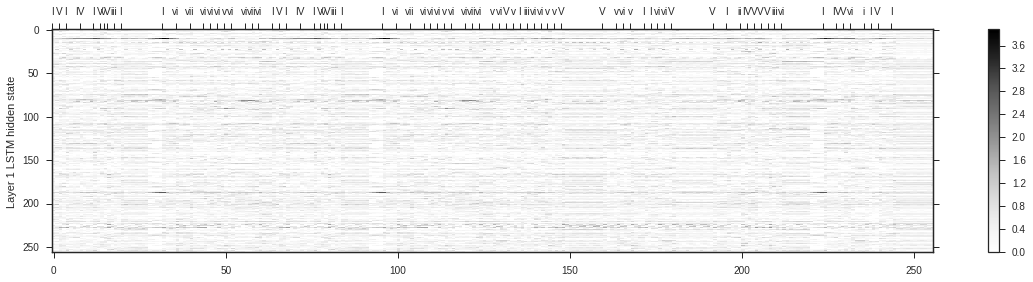
\includegraphics[width=1.0\linewidth]{Figures/model-analysis-chords-1.png}
    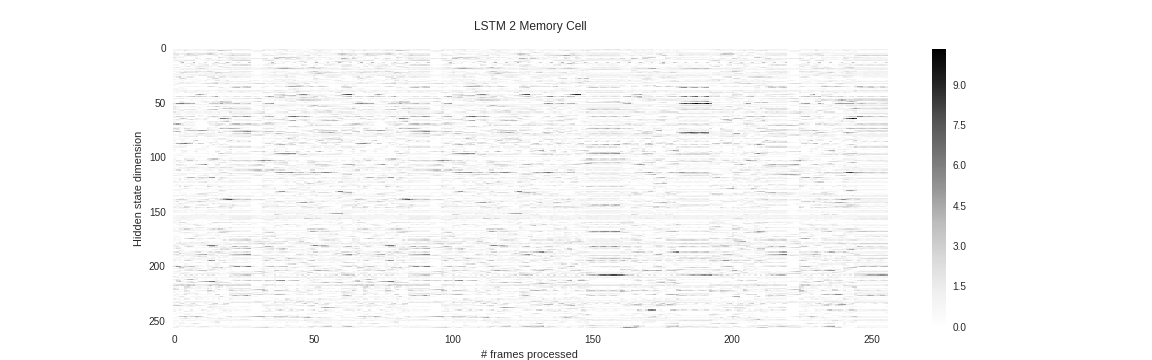
\includegraphics[width=1.0\linewidth]{Figures/model-analysis-chords-2.png}
    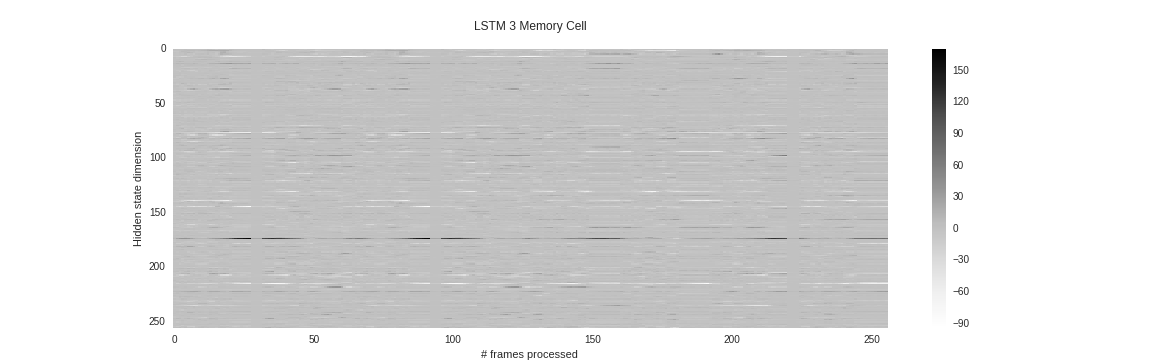
\includegraphics[width=1.0\linewidth]{Figures/model-analysis-chords-3.png}
    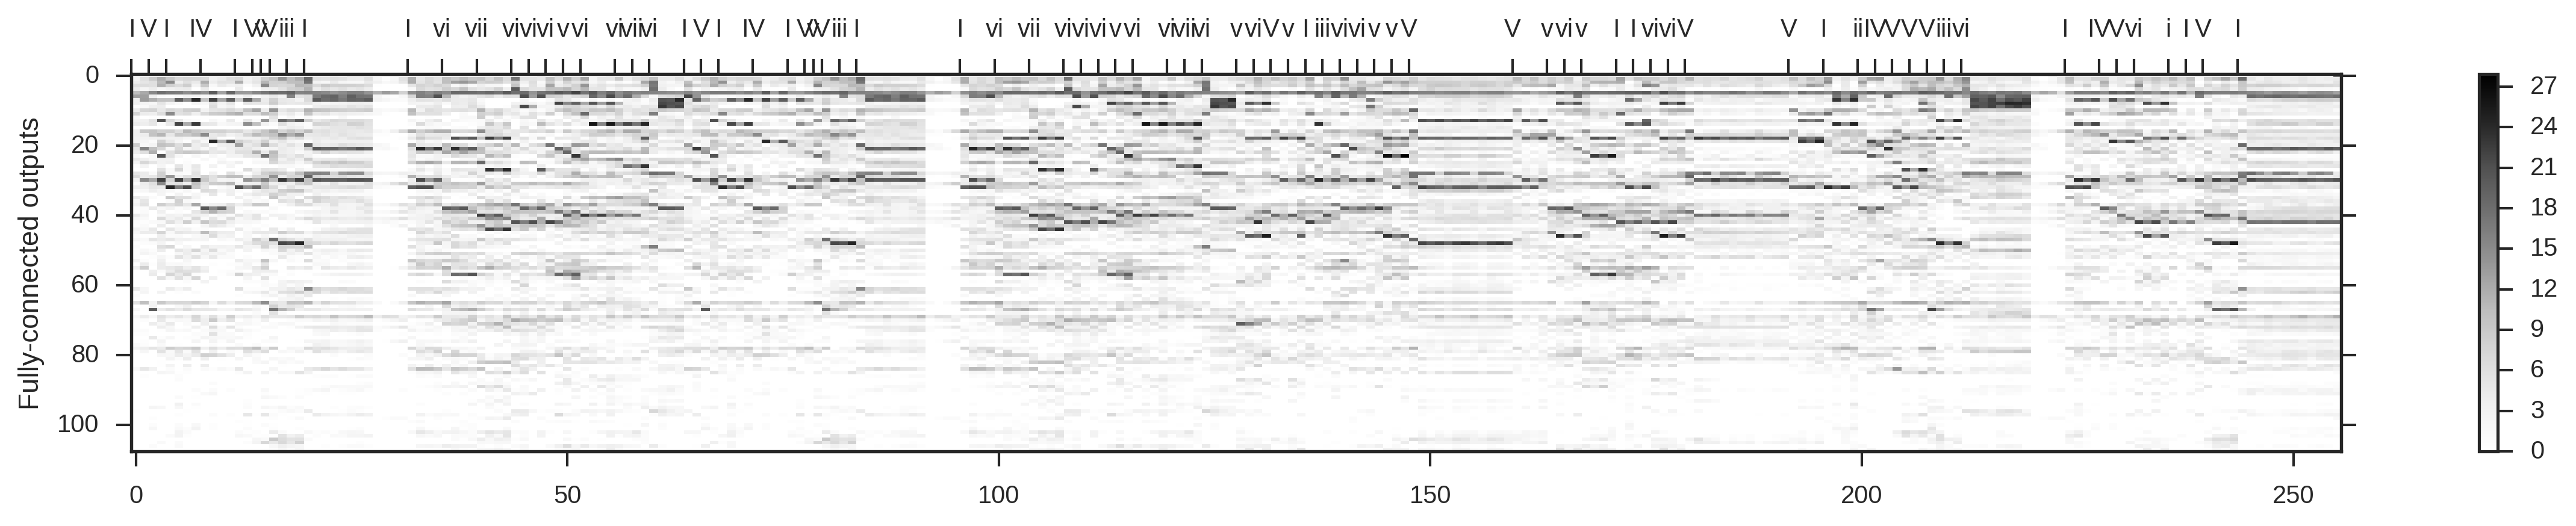
\includegraphics[width=1.0\linewidth]{Figures/model-analysis-chords-4.png}
    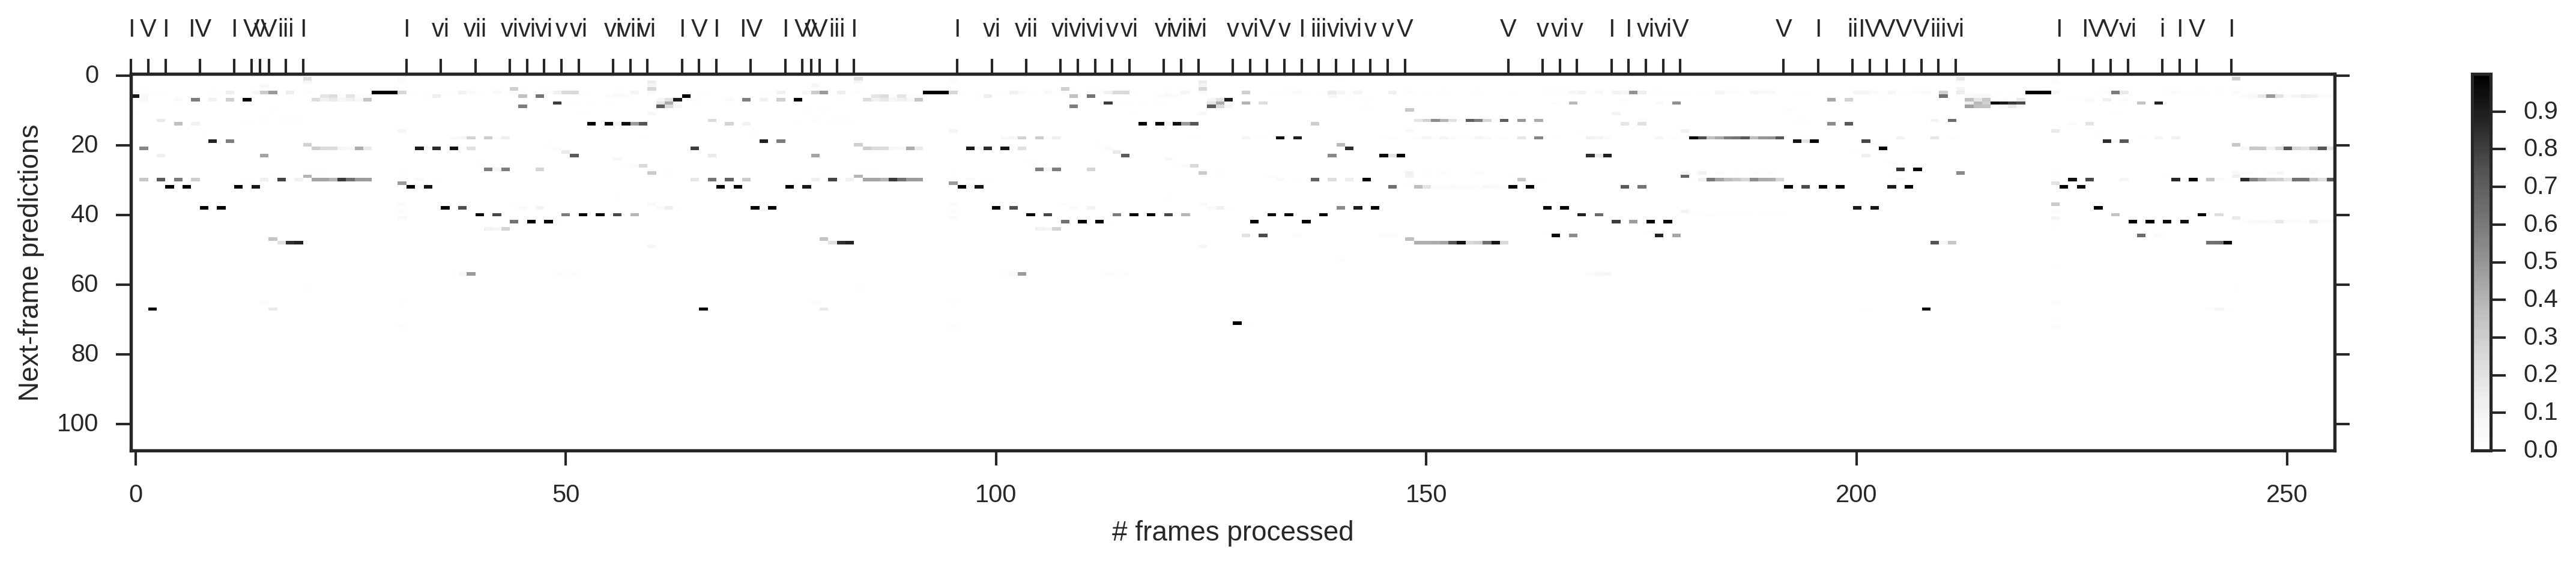
\includegraphics[width=1.0\linewidth]{Figures/model-analysis-chords-5.png}
    \caption{}
    \label{fig:}
\end{figure}

Probabilistic piano roll
\begin{figure}[htpb]
    \centering
    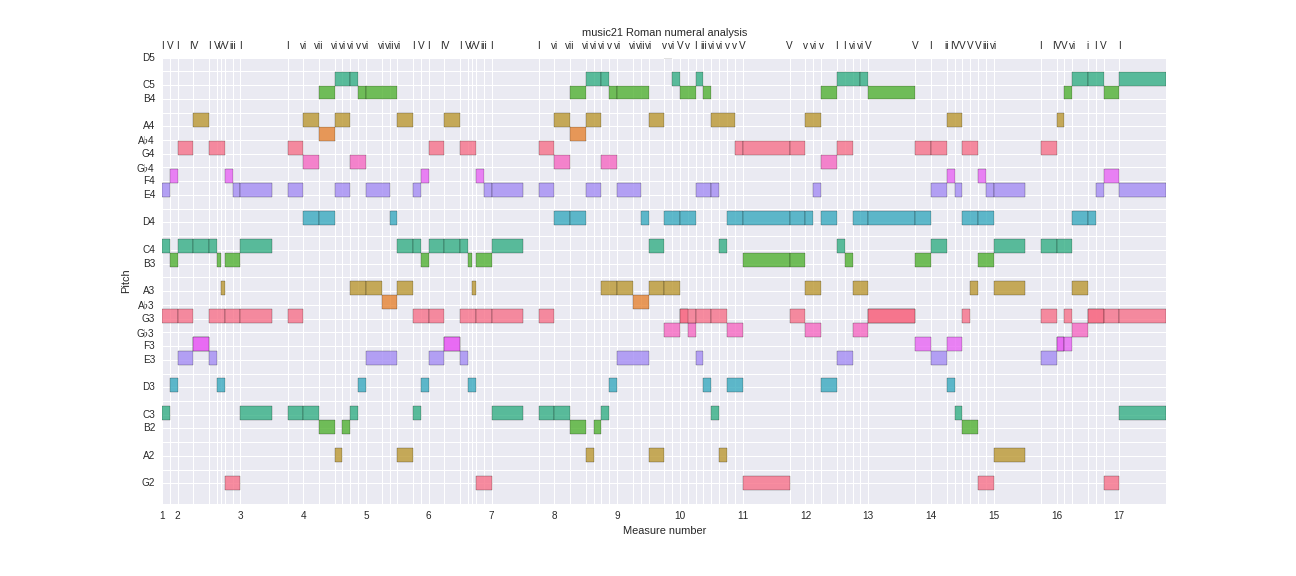
\includegraphics[width=1.0\linewidth]{Figures/model-analysis-input-piano-roll.png}
    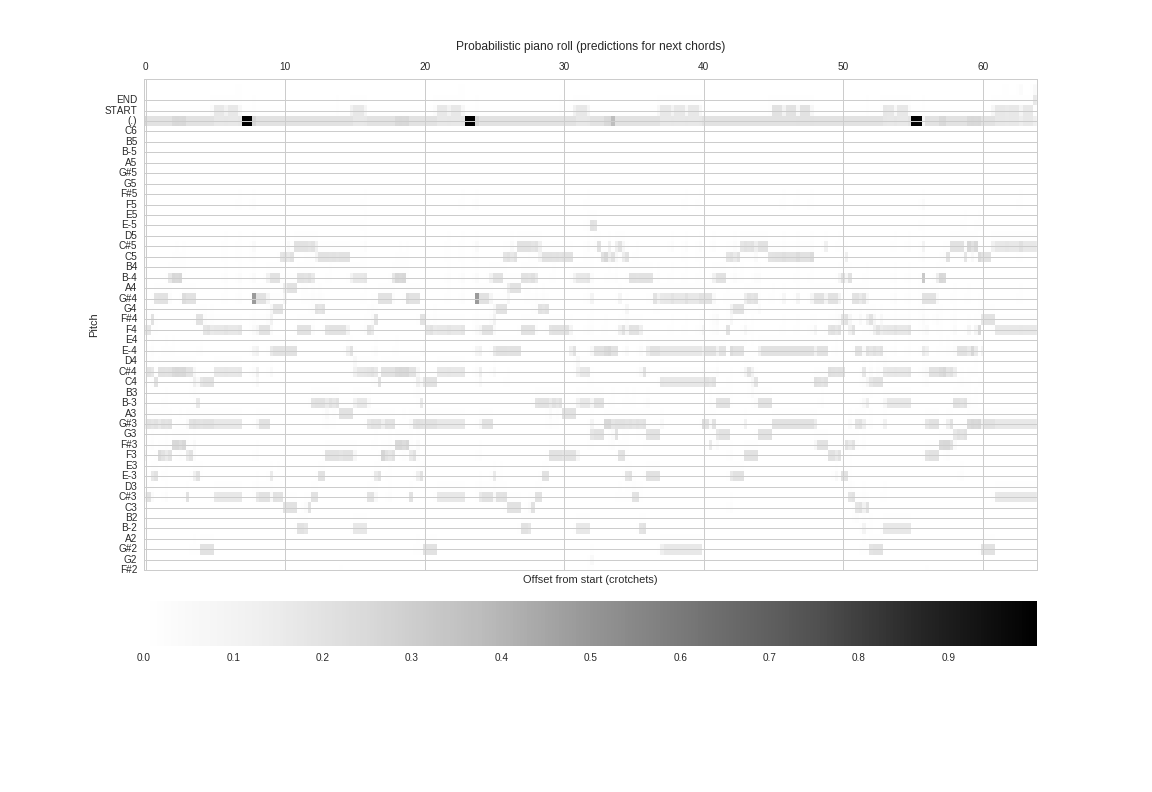
\includegraphics[trim={0 0 0 1.4cm},clip,width=0.995\linewidth]{Figures/model-analysis-probabilistic-piano-roll.png}
    \caption{Figures/model-analysis-probabilistic-piano-Roll}
    \label{fig:Figures/model-analysis-probabilistic-piano-roll}
\end{figure}

\subsection{Interesting neurons}

\begin{figure}[htpb]
    \centering
    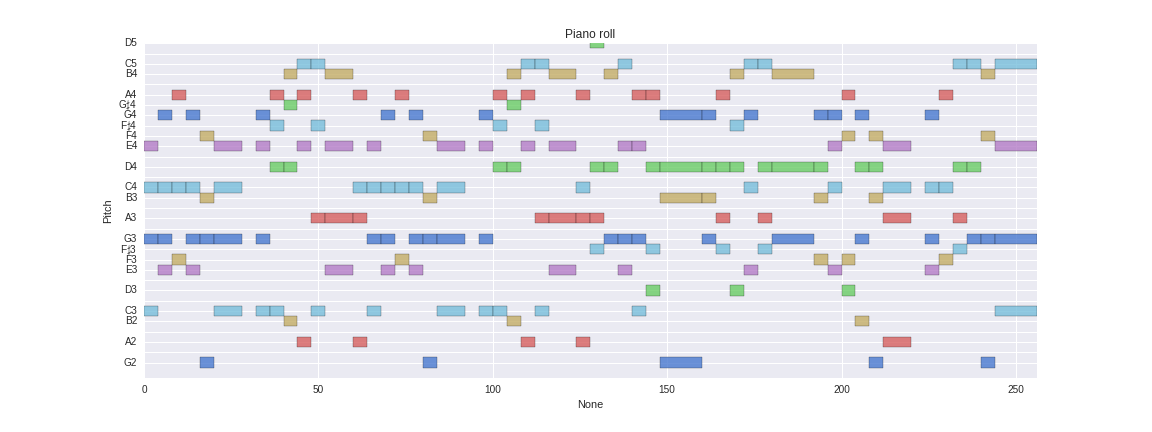
\includegraphics[width=1.0\linewidth]{Figures/model-analysis-cells-softmax-piano-roll.png}
    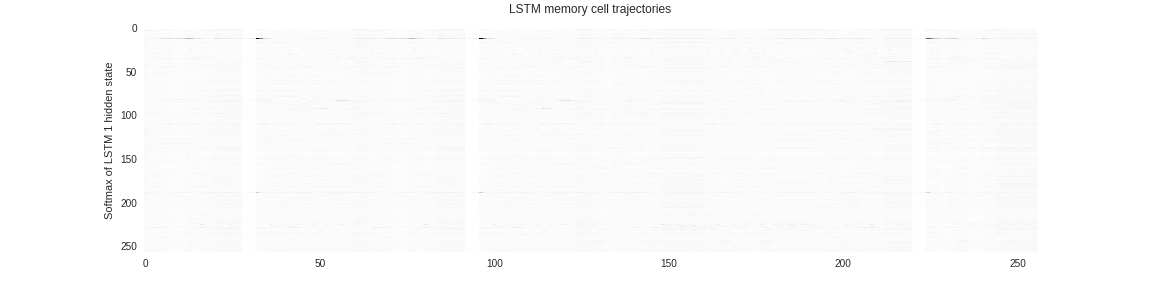
\includegraphics[width=1.0\linewidth]{Figures/model-analysis-cells-softmax-1.png}
    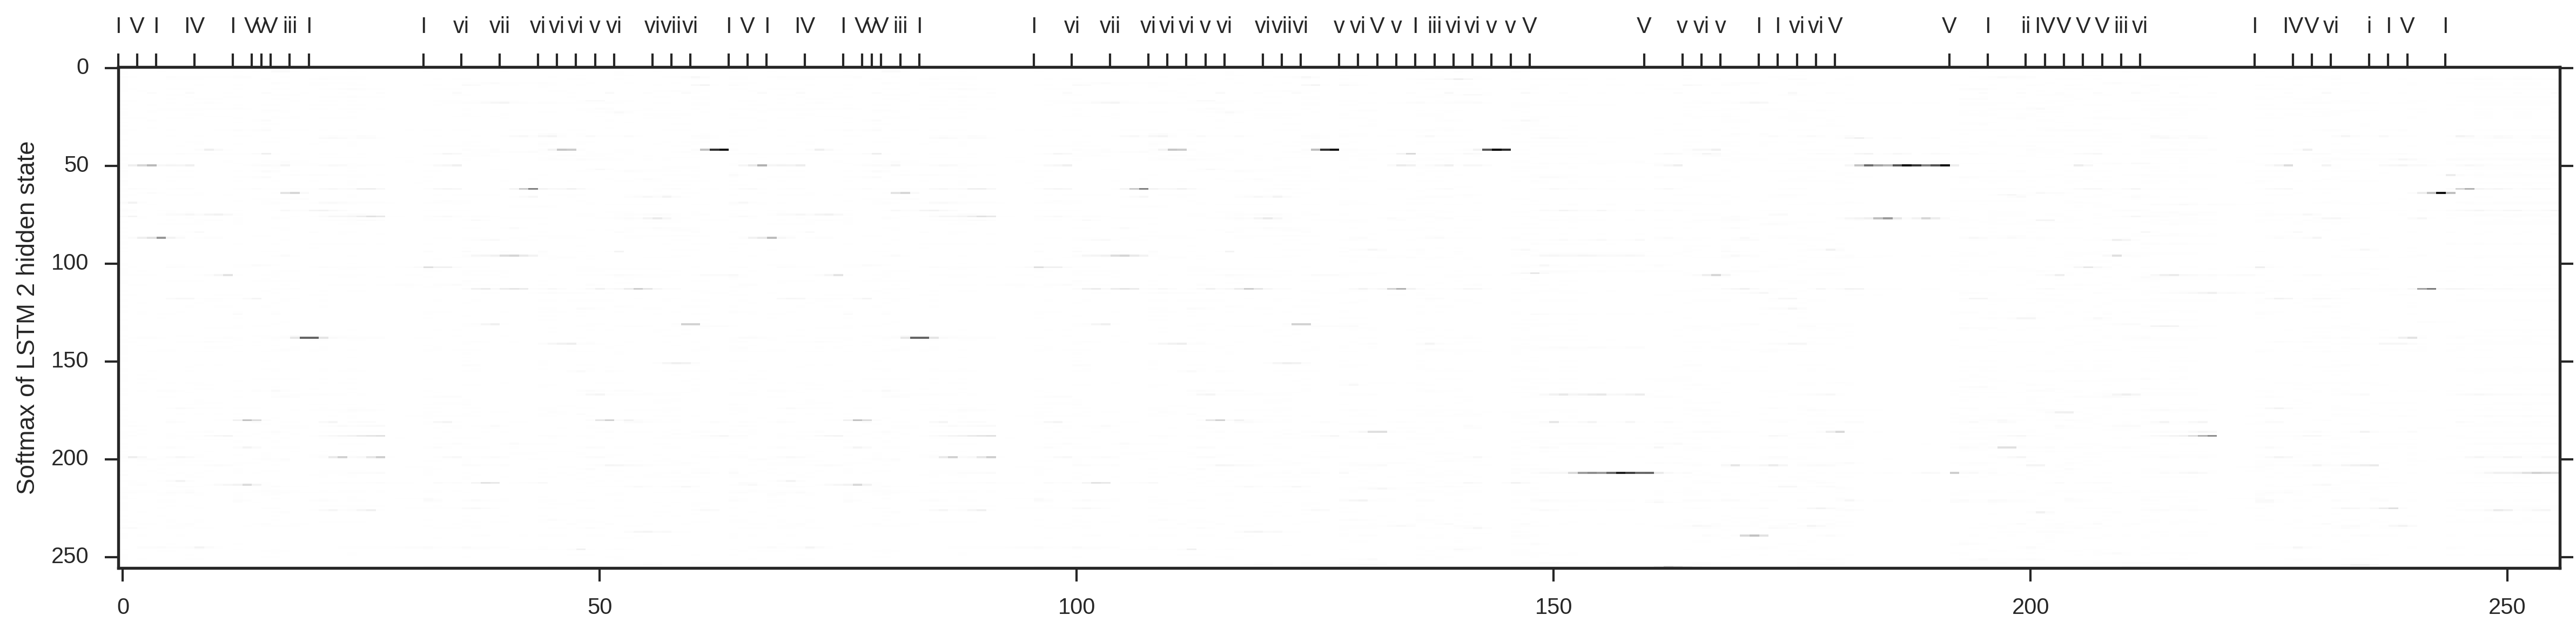
\includegraphics[width=1.0\linewidth]{Figures/model-analysis-cells-softmax-2.png}
    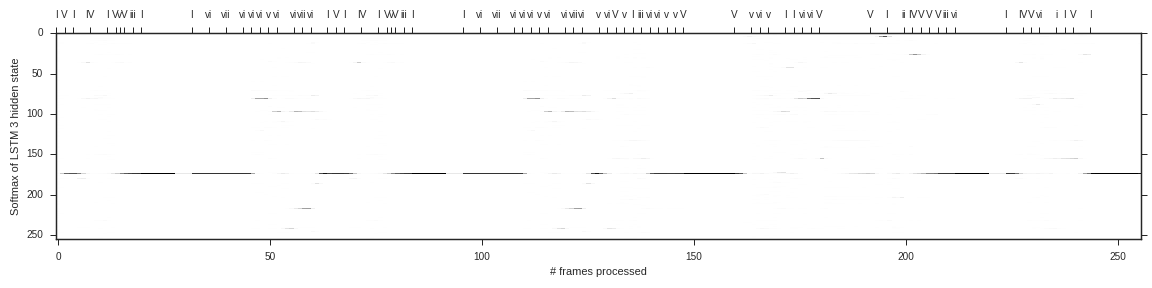
\includegraphics[width=1.0\linewidth]{Figures/model-analysis-cells-softmax-3.png}
    \caption{model-analysis-cells-Softmax}
    \label{fig:model-analysis-cells-softmax}
\end{figure}

\begin{figure}[htpb]
    \centering
    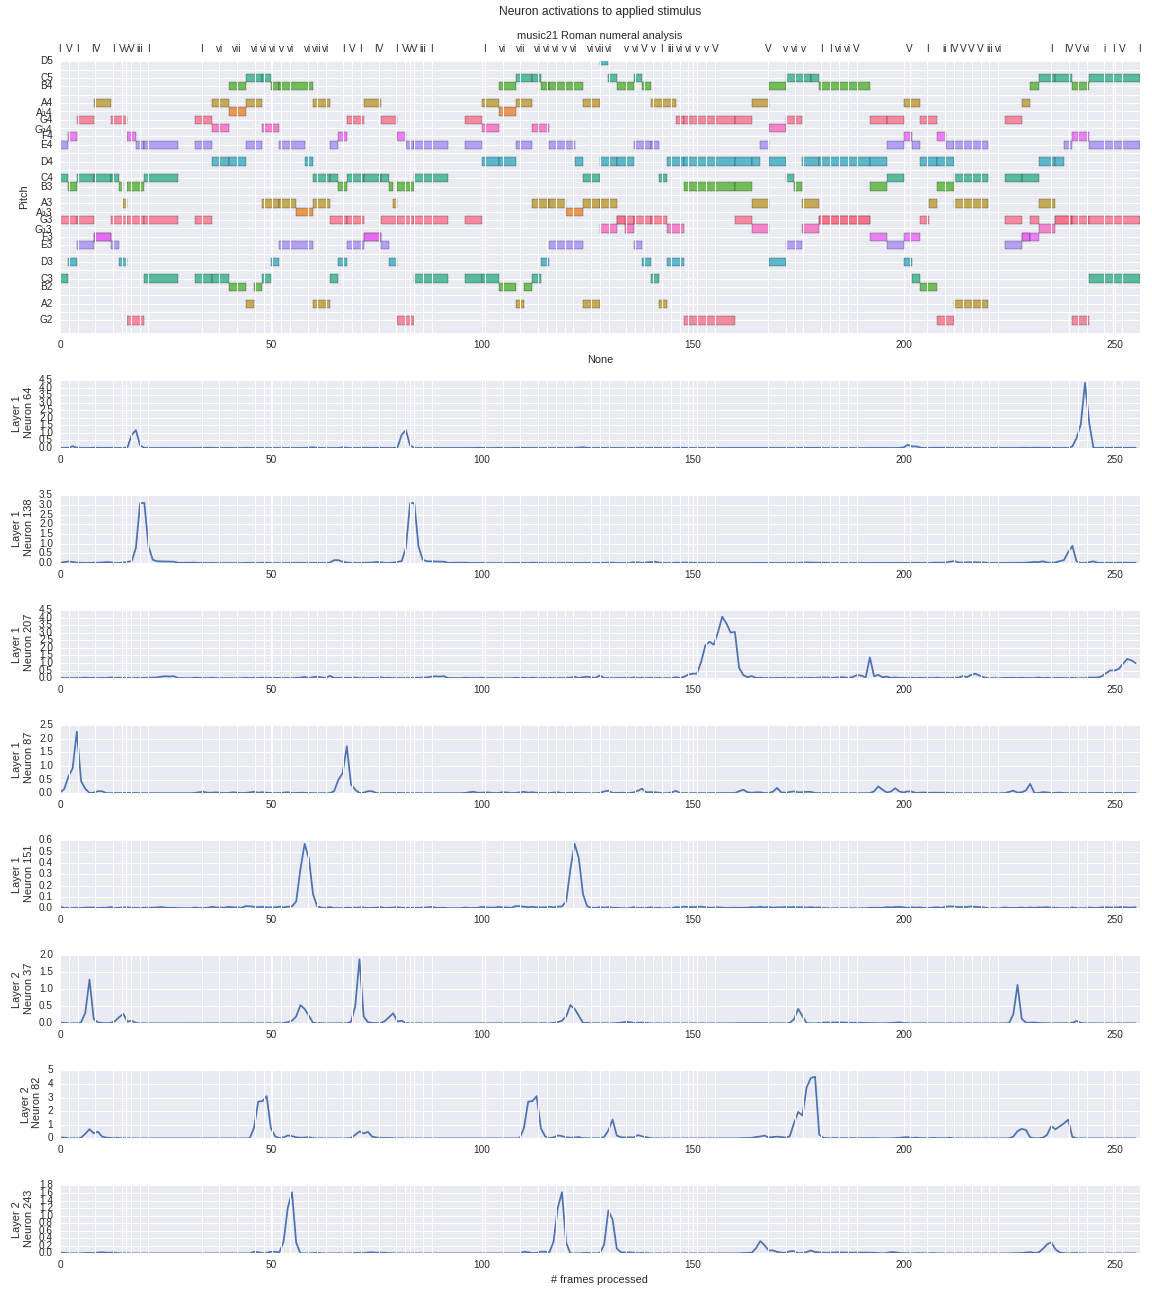
\includegraphics[width=1.0\linewidth]{Figures/model-analysis-cells-individual.png}
    \caption{Figures/model-analysis-cells-Individual}
    \label{fig:Figures/model-analysis-cells-individual}
\end{figure}


\printbibliography

\end{document}
